\documentclass[12pt]{article}

\usepackage[utf8]{inputenc}
\usepackage[brazil]{babel}
\usepackage{graphicx}
\usepackage[table]{xcolor}
\usepackage{tabularx}
\usepackage{hyperref}
\usepackage{booktabs}
\usepackage{bookmark}

\begin{document}
\title{TerraCota\\Game Design Document}
\author{NullPointer Corporation}
\date{v0.3}
\maketitle

\newpage

\begin{table}[h]
  \centering
  \begin{tabular}{ccll}
    \toprule
    \textbf{Versão} & \textbf{Data} & \textbf{Autor} & \textbf{Descrição} \\
    \midrule
    0.1 & 22/04/2015 & Carlos Oliveira  & Versão Inicial \\
    \rowcolor[gray]{0.9}
    0.2 & 20/05/2015 & Álvaro Fernando & Adicionando novas seções \\
    0.3 & 22/05/2015 & Carlos Oliveira & Front-end \\
    \rowcolor[gray]{0.9}
    0.4 & 30/05/2015 & Álvaro Fernando & Objetos Colecionáveis \\
    \bottomrule
  \end{tabular}
  \caption{Histórico de Revisões}
\end{table}

\newpage

\tableofcontents

\newpage

\listoffigures

\newpage
\section{Objetivo do jogo}

\subsection{Conceito do jogo}
O jogo terá uma movimentação semelhante a games do estilo beat'em up (briga de
rua em português), como principais referências e exemplos os jogos Little
Fighter 2 (PC), Captain Commando (SNES), Double Dragon (SNES).

A temática será a de um mundo pós-apocalíptico, onde várias tecnologias se
extinguiram e a humanidade volta a comunicar-se de forma arcaica por meio de
figuras e indicações corporais. O jogador terá que, entre outros desafios,
resolver puzzles decifrando códigos audiovisuais para completar as quests.

Todos os membros da equipe estão cientes do conceito do jogo. No diretório
deste arquivo é possível visualizar algumas imagens feitas pelo artista Pedro
Braga que podem auxiliar no entendimento da temática.

\subsection{Principais características}
Uma das características mais interessantes do jogo são o modo como os gêneros
aventura e puzzle interagem entre si, fazendo com o que o jogador precise
pensar e decifrar qual será sua missão, pois as informações serão dadas
através de símbolos.

A movimentação é em dois eixos, vertical e horizontal, mais do que um jogo de
plataforma, que contém só um, desconsiderando a função de pular, também é uma
característica diferenciada do jogo, pois traz um modo de exploração em visão
em múltiplos planos. A inspiração desse estilo de movimentação veio,
principalmente, do jogos Capitão Comando, Little Fighter 2 e Double Dragon.

Não estará presente no jogo elementos relacionados à economia e/ou obtenção de
recursos, tais como dinheiro, moeda, cristais, etc. Levando em consideração o
conceito do jogo, a humanidade se abstém de um sistema monetário, colocando em
prática a barganha para obtenção de itens, peças, alimentos, etc.

\section{Visão geral}
O jogo é dividido em 5 segmentos, ou 5 capítulos:
\begin{enumerate}
\item Tutorial pra interação com o mundo, tarefas simples como "ir falar com o
carteiro" ou "buscar o leite na despensa" para o jogador se acostumar com a
linguagem do jogo. Este tutorial será exibido na forma de uma cutscene, dessa
forma não haverá interação do usuário.
Após essa pequena introdução é revelado que alguns morcegos/monstros invadiram
o último andar da torre, e o jogador deve ir se livrar deles.

\item O jogador precisa de alguma arma, então deve ir até o ferreiro para
conseguir uma espada simples. Ele sobe até o último andar da torre e elimina os
morcegos, mas por acidente desperta o mecanismo de defesa da torre, que o ataca
(chefão 1).
Durante a batalha, a espada do Inti se prova ineficaz (pode talvez quebrar)
porém ele acha uma espada fincada na parede próxima ao chefão. Ele remove a
espada (o que destranca a porta para a saída pro mundo afora) e usa ela pra
derrotar o chefão.
Ao derrotar o chefão uma porta atrás dele se revela e abre, revelando um mundo
inteiro do lado de fora.

\item Curioso pra explorar o mundo, Inti sobe no "elevador" do lado de fora da
torre e desce para o chão, entrando numa floresta.
Ao caminhar pela floresta ele encontra a Killa, sentada em um galho. Ela percebe
ele, sorri, chama ele e sai andando. A missão se torna seguir a Killa.
Ela guia ele até a aldeia dela, e introduz o pai dela (cacique) e o jogador se
torna livre a explorar os arredores e a realizar sidequests (se der tempo de
desenvolvê-las), a missão se torna retornar à torre e contar para os pais sobre
a existência de mais pessoas além das que vivem na torre com ele.

\item Ele retorna para a torre, Killa fica para trás porque o pai dela não deixa
ela sair da floresta, e tenta convencer as pessoas sobre o mundo de fora. Ninguém
acredita nele nem segue ele quando ele tenta mostrar. Ele decide procurar um
artefato valioso pra provar a existência do mundo lá fora (estamos pensando em
fazer um artefato que seja presente em toda torre, porém só um. Ao trazer um de
outra torre ele prova a existência dela).
Então ele volta para a floresta e Killa se junta a ele mais uma vez, e ajuda ele
a chegar na torre onde ela vivia. Numa região alagada da floresta. Os dois
entram na torre.

\item A torre abandonada, cheia de puzzles. Ao chegar na câmara onde o artefato
está, eles percebem que precisam de uma chave pra destrancar ela. Quando eles
encontram a chave, o chefão a engole antes que eles consigam pegar ela. O objetivo
se torna derrotar o chefão pra pegar a chave de volta, e então conseguir o artefato.
Com o artefato em mãos, o Inti volta pra torre, prova a existência do mundo afora,
e o jogo termina com a população na frente da porta, olhando o mundo do lado de fora
\end{enumerate}

\section{Requisitos Tecnológicos}

\subsection{Ferramentas de codificação}
O jogo Terracota será desenvolvido na linguagem de programação C++, linguagem
esta de uso geral e caracterizada pelo versatilidade e alto desempenho. Bastante
usada no setor de jogos eletrônicos. Para compilação do código será utilizado o
Clang, versão 3.4.Os editores de texto utilizados para a codificação serão o Vim
(open-source) e o Sublime-Text (proprietário).

Os sistemas operacionais utilizados serão Ubuntu 14.04, Windows 8 e Mac OS X.

\subsection{Ferramenta de controle de versão}
A equipe irá utilizar como ferramenta de versionamento do código o {\bf Git}.
Nela é possível criar uma cópia bem mais rápido que outras ferramentas de
controle de versão, é otimizada para funcionar na internet, seus repositórios
ocupam menos espaços, é mais fácil de administrar diferentes fontes de
modificações, permitindo um melhor fluxo de trabalho.

\subsection{Ferramentas gráficas e de áudio}
Para a codificação, será utilizado a biblioteca multimídia livre escrita em C
{\bf SDL2}. Para o desenvolvimento da arte final do jogo, será utilizado os
programas da empresa Adobe, Photoshop CC Fotografia e Ilustrator CC.

Para o áudio, OpenAL. É uma API livre , multiplataforma desenvolvida pela empresa
Loki Software para lidar com áudio multicanal tridimensional, é usado normalmente
com o OpenGL.As funcionalidades da biblioteca são baseadas em três conceitos:
objetos que emitem som, som que será mantido por algum objeto e ouvinte da cena.

\subsection{Ferramentas de rede}
O Terracota {\bf não} terá suporte à multijogadores em rede, seja local ou online.

\section{Controles}
Esta seção trata dos controles do jogo e sua respectiva ação/movimento. Para
o mecanismo de movimentação pelo mundo será utilizado apenas os movimentos
corporais do protagonista. Por tanto não haverá {\bf veículos} no jogo.

\subsection{Lista de movimentos}
O personagem poderá se movimentar da seguinte maneira:

\begin{itemize}
    \item Baixo
    \item Cima
    \item Direita
    \item Esquerda
    \item Interação
    \begin{itemize}
        \item Ação especial
        \begin{itemize}
            \item Empurrar bloco; ou
            \item Escalar
        \end{itemize}
        \item Conversar com NPC
        \item Pegar item
    \end{itemize}
    \item Ataque
\end{itemize}

\subsection{Esquema básico com teclado}
\begin{itemize}
    \item \textbar W\textbar \textbar A\textbar \textbar S\textbar \textbar D\textbar - Movimentação
    \item \textbar ESC\textbar - Voltar (nos menus)
    \item \textbar E\textbar \textbar N\textbar - Interação
    \item \textbar SPACE\textbar - Atacar
    \item \textbar C\textbar - Trocar personagem
    \item \textbar ESC\textbar \textbar P\textbar - Pause (durante jogo)
\end{itemize}

\subsection{Esquema com o controle de PS4}
\begin{itemize}
    \item \textbar SETAS DIRECIONAIS\textbar - movimentação
    \item \textbar BOLA\textbar - Voltar (nos menus)
    \item \textbar QUADRADO\textbar - Atacar
    \item \textbar X\textbar - Interação
    \item \textbar X\textbar - Selecionar (nos menus)
    \item \textbar TRIÂNGULO\textbar - Trocar personagem
    \item \textbar OPTIONS\textbar - Pause(durante jogo)
\end{itemize}

\subsection{Esquema com o controle de Xbox 360}
\begin{itemize}
    \item \textbar SETAS DIRECIONAIS\textbar - movimentação
    \item \textbar A\textbar - Interação
    \item \textbar X\textbar - Atacar
    \item \textbar B\textbar - Interagir
    \item \textbar Y\textbar - Trocar personagem
    \item \textbar START\textbar - Pause(durante jogo)
\end{itemize}

\section{Saúde}

\subsection{Aspectos Gerias}
Cada personagem (Inti e Killa) terá sua própria barra de vida. Elas serão
exibidas no canto superior esquerdo da tela.


A barra de vida/saúde terá 9 espaços {\bf sem} divisões visíveis entre eles.
Se um dos personagens tiver a vida esgotada, ele ficará incapacitado (por exemplo,
não poderá atacar).


Após 30 segundos, a vida recarrega 3 espaços.

\subsection{Estados anormais}
O jogo não terá estados anormais de saúde das personagens.

\subsection{Vidas}
O aspecto principal da saúde das personagens no jogo será a barra de saúde.
Não haverá acumulo de vidas como os conceitos relacionados ao cogumelo verde
do Mario.

\subsection{Morte}
Quando a barra de vida/saúde dos dois personagens se extinguir, a tela de
sinalizando o fim do jogo irá aparecer e o jogador terá as opções do menu
principal novamente expostas, com uma opção de voltar à um ponto anterior
ao da morte.

\section{NPCs}
O jogo terá cinco NPCs (non-player character - personagem não jogável):
\begin{enumerate}
\item Mãe do personagem Inti:
\subitem {\bf Nome:} desconhecido;
\subitem {\bf Sexo:} feminino;
\subitem {\bf Idade:} +40;
\subitem {\bf Background:} mãe amorosa;
\subitem {\bf Nível onde será encontrada:} primeiro nível, primeiro andar da
primeira torre;
\subitem {\bf Diálogos:} (não definidos);
\subitem {\bf Colisão:} jogador aciona tecla/botão de interação para iniciar a
colisão;
\subitem {\bf Recompensas:} diz palavras/símbolos carinhosos ao Inti.

\item Pai de Inti:
\subitem {\bf Nome:} desconhecido;
\subitem {\bf Sexo:} masculino;
\subitem {\bf Idade:} +40;
\subitem {\bf Background:} pai forte, como é preciso ser no mundo
pós-apocalíptico;
\subitem {\bf Nível onde será encontrada:} primeiro nível, primeiro andar da
primeira torre;
\subitem {\bf Diálogos:} (não definidos);
\subitem {\bf Colisão:} jogador aciona tecla/botão de interação para iniciar a
colisão;
\subitem {\bf Recompensas:} diz palavras/símbolos de força ao Inti.

\item Pessoa que dá a quest/missão de matar os morcegos:
\subitem {\bf Nome:} desconhecido;
\subitem {\bf Sexo:} (não definido);
\subitem {\bf Idade:} +20;
\subitem {\bf Background:} (não definido);
\subitem {\bf Nível onde será encontrada:} (não definido);
\subitem {\bf Diálogos:} dirá por meio de símbolos que Inti deve matar os
morcegos que atormentam os moradores da torre;
\subitem {\bf Colisão:} jogador aciona tecla/botão de interação para iniciar a
colisão;
\subitem {\bf Recompensas:} entrega quest.

\item O Ferreiro
\subitem {\bf Nome:} desconhecido;
\subitem {\bf Sexo:} masculino;
\subitem {\bf Idade:} +50;
\subitem {\bf Background:} (não definido);
\subitem {\bf Nível onde será encontrada:} primeiro nível, primeiro andar da
primeira torre;
\subitem {\bf Diálogos:} homem de poucas palavras, diz apenas símbolos de "eu
tenho muito trabalho à fazer";
\subitem {\bf Colisão:} jogador aciona tecla/botão de interação para iniciar a
colisão;
\subitem {\bf Recompensas:} entrega espada ao Inti para matar os morcegos.

\item Pai da Killa
\subitem {\bf Nome:} desconhecido;
\subitem {\bf Sexo:} masculino;
\subitem {\bf Idade:} +40;
\subitem {\bf Background:} (não definido);
\subitem {\bf Nível onde será encontrada:} vila fora das torres;
\subitem {\bf Diálogos:} (não definido);
\subitem {\bf Colisão:} jogador aciona tecla/botão de interação para iniciar a
colisão;
\subitem {\bf Recompensas:} entrega quest/missão para segunda torre.
\end{enumerate}

\section{Front-End}
Esta seção apresenta as telas que são exibidas no início do jogo. As seguintes
imagens são apresentadas no decorrer da abertura do jogo.

\subsection{Logotipo da empresa}

\begin{figure}[!htb]
    \centering
    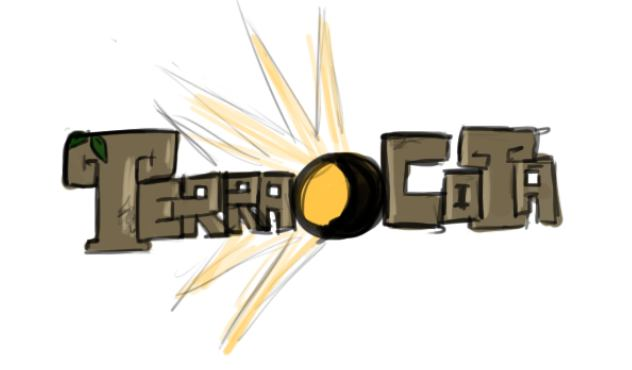
\includegraphics[scale=0.5]{logo-terracota.jpg}
    \caption{Logotipo Terracota}
    \label{fig:terracota_logo}
\end{figure}

\subsection{Softwares de Terceiros}

\begin{figure}[!htb]
    \centering
    
\includegraphics[scale=0.2]{logo-sdl.png}
    \caption{Logotipo SDL}
    \label{fig:sdl_logo}
\end{figure}

\subsection{Requisitos legais}

\begin{figure}[!htp]
    \centering
    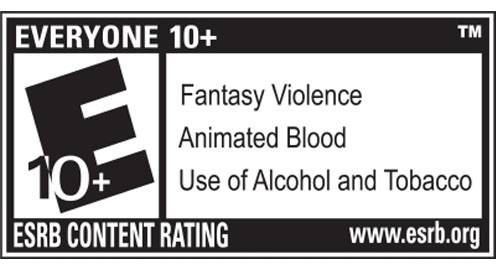
\includegraphics[scale=0.3]{faixa_etaria.jpg}
    \caption{Faixa indicativa}
    \label{fig:faixa_indicativa}
\end{figure}

\section{Objetos Colecionáveis}
Esta seção contempla a descrição dos objetos colecionáveis do jogo.

\subsection{Primeira Espada}
Encontrada no primeiro nível, recebida do NPC Ferreiro. Possibilita ao jogador
o movimento de ataque.

\begin{figure}[!htb]
    \centering
    
\includegraphics[scale=0.5]{sword1.png}
    \caption{Primeira Espada}
    \label{fig:primeira_espada}
\end{figure}

\subsection{Segunda Espada}
Encontrada na segunda torre, na qual mora Killa. Recebida após encontrar
um baú de tesouro nesta torre. Possibilita ao jogador o movimento de ataque.

\begin{figure}[!htb]
    \centering
    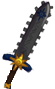
\includegraphics[scale=0.5]{sword2.png}
    \caption{Segunda Espada}
    \label{fig:segunda_espada}
\end{figure}

\end{document}
